\documentclass[12pt,titlepage]{article}

\usepackage{ctex}
\usepackage{graphicx}
\usepackage{amsmath}
\usepackage{booktabs}
\usepackage{threeparttable}
\usepackage[colorlinks,allcolors=black]{hyperref}

\title{建立一种用于动态预测脓毒症患者\\诱发 PICS 的机器学习方法}
\author{%
华东理工大学\\
白栋栋\ 成昊南\ 黄海骅\ 霍松泽%
}
\date{}

\begin{document}


\maketitle


\begin{abstract}
    \hspace{\parindent}PICS 会导致脓毒症患者长期死亡率增加,%
    因而适当合理地预测患者诱发 PICS 的几率尤为重要。%
    本研究通过开发和验证机器学习模型,以动态预测重症脓毒症患者的 PICS 风险为目的,%
    基于 eICU 协作研究数据库\nobreak(eICU CRD),开发并验证机器学习模型。%
    通过数据分析,在最终提取的 $100,308$ 条数据中,有 $3866$ 条数据为正例,%
    即 $3.85\%$ 的数据所对应的患者诱发了 PICS 。我们训练了完整模型和紧凑模型,%
    能够动态预测脓毒症患者诱发 PICS 的风险,优于传统的 logistic 回归,%
    并且其中紧凑模型明显在临床上更加可行、更加易用。为了方便使用,%
    还开发了 H5 网页用于便捷预测患者发生 PICS 的概率,是本研究的创新之处。

    \noindent\textbf{关键词:}脓毒症,PICS,eICU,机器学习,Catboost 模型
\end{abstract}


\tableofcontents
\newpage


\section{项目背景}

脓毒症是宿主应对感染出现炎症反应失调引起的器官功能损伤,表现为危及生命的一组临床综合征。%
脓毒症患者的病死率较高,是感染引起患者死亡的主要原因\textsuperscript{\cite{sepsis}}。%
而脓毒症将会诱发 PICS(持续炎症-免疫抑制-分解代谢综合征),%
这是部分患者在度过脓毒症急性期乃至出院后,仍处于慢性持续炎症、免疫功能抑制以及高分解代谢状态的症状。%
PICS 早期即具有明显的炎症反应和免疫抑制反应,后来转化为持续性炎症和免疫抑制状态,%
出现进行性的器官损伤以及持续的肌肉质量丧失、伤口愈合不良和呼吸机依赖等,且还会导致器官功能障碍,%
生活质量下降,可能需要长期的医疗监护\textsuperscript{\cite{pics}}。%
所以,若可以帮助临床上及时、准确地预测可能发生的 PICS 状况,并及时采取相应治疗手段,%
可减轻病患痛苦,增加患者痊愈的概率。

PICS 概念自 2012 年提出以后,其诊断标准经过 2015 年及 2017 年的改进,%
目前包括以下 $4$ 个方面:

\begin{enumerate}
    \item[(1)] ICU 住院天数 $\ge 14~\text{天}$;
    \item[(2)] 持续的炎症反应:C 反应蛋白 $\ge 150~\text{mg/L}$ ,\
        视黄醇结合蛋白 $< 10~\text{mg/L}$ ;
    \item[(3)] 免疫抑制:淋巴细胞计数 $\le 0.80 \times 10^{9}~\text{/L}$ ;
    \item[(4)] 分解代谢:血清白蛋白 $< 30$ g/L ,肌酐/身高指数 $< 80\%$ ,\
        住院期间体重下降 $ > 10\%$ 或身体质量指数 $< 18~\text{kg/m\textsuperscript{2}}$ 。
\end{enumerate}

尽管这些临床标志物不是对炎症、免疫抑制或分解代谢的直接测量,但其方便获取,%
可以作为重症监护室医务人员评估患者临床状况的依据\textsuperscript{\cite{pics-conditions}}。%
除了以降钙素原、C 反应蛋白和白介素-6等传统生物标志物作为疾病评估和预后的指标外,%
近年关于 microRNAs 作为生物标志物用于组织损伤、炎症等多种疾病的研究也成为热点。%
microRNA 参与了脓毒症后炎症反应及内皮细胞功能调节,可用于判断脓毒症后所处阶段,%
进而有利于评估 PICS 患者的预后。目前已被证实,可用于评估预后的 microRNAs 包括 miR-146a、%
miR-125b 及 miRNA-155 等\textsuperscript{\cite{micro-rna}}。%
同时,亦有研究采用 APACHE-Ⅱ 评分、住 ICU 时间、CD4+/CD8+ 比值、%
机械通气 4 项独立危险因素构建的预测模型,预测脓毒症患者 PICS 的发生情况%
\textsuperscript{\cite{pics-prediction-methods}}。


\section{材料和方法}

\subsection{数据来源}

我们主要基于一个大型重症监护数据库进行了这项研究,这个数据库是 eICU 协作研究数据库%
(eICU-Collaborative Research Database, eICU-CRD)。%
该数据库由美国麻省理工学院和飞利浦医疗保健公司联合提供,%
是包含了 $200$ 多家医院的 $335$ 个监护室中, $20$ 多万条患者医学信息的数据集\textsuperscript{\cite{eicu}}。%
而它的 2.0 版本则涵盖了 2014 年至 2015 年全美 $208$ 家医院入住重症监护病房的 $139,367$ 名患者的常规数据,%
共 $200,859$ 条住院记录。两位作者访问了这个数据库,并负责数据提取处理,为后续开展研究做准备。

\subsection{选择数据}

统计病人在脓毒症住院期间的临床和测试变量,对于一些具有多个测量值的变量,估计其平均值。%
为了预测 PICS ,我们收集了 $57$ 个变量,包括患者的特征(年龄、性别、种族和住院类型)、%
生命体征(呼吸频率、血压、心率、血氧和体温)、测试数据(血气、常规血液分析、肝功能、肾功能和凝血特征)、%
输血量(红细胞、血小板和新鲜冷冻血浆)和尿量。

\subsection{研究方法}

\begin{figure}[htb]
    \centering
    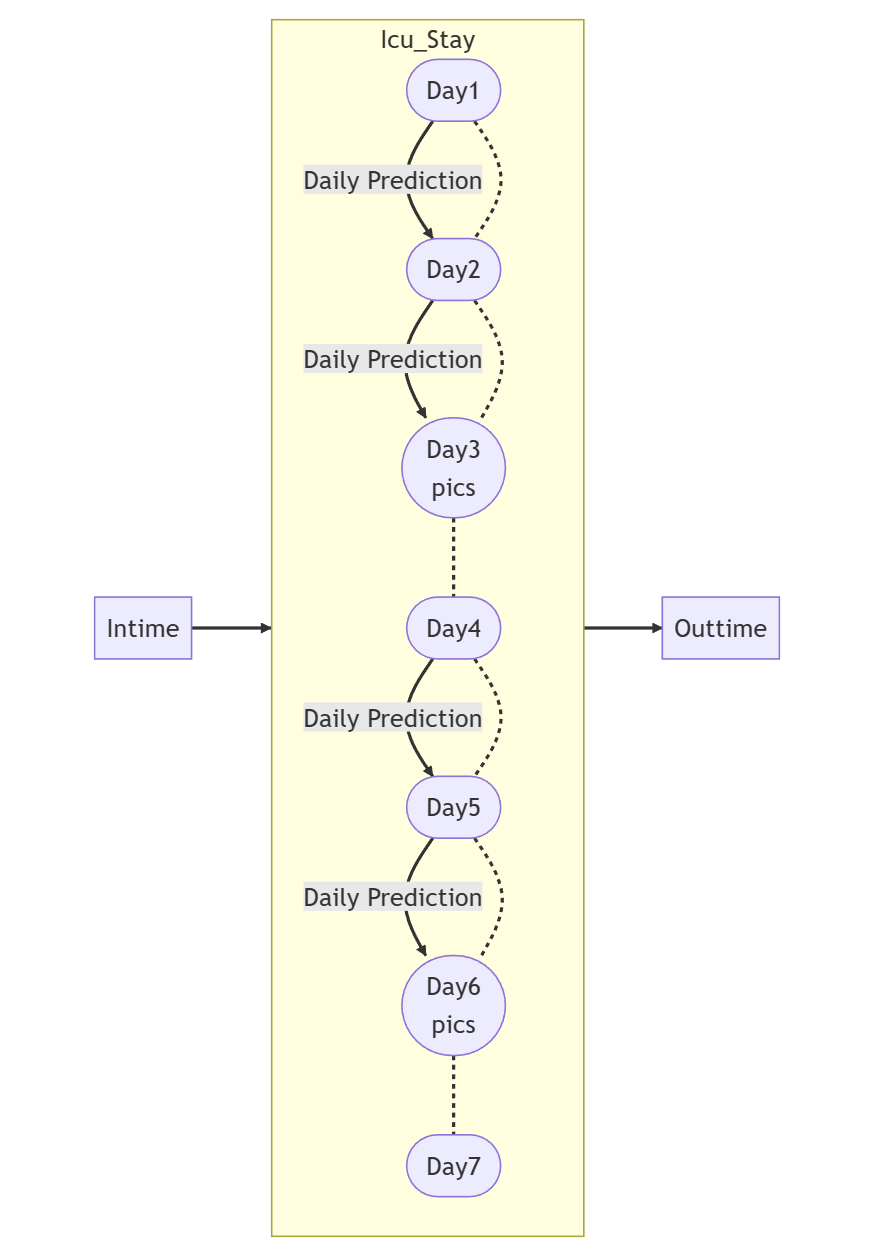
\includegraphics[width=0.6\linewidth]{../img/predicting.png}
    \caption{动态预测 PICS 示意图}
    \label{fig:predicting}
\end{figure}

如图 \ref{fig:predicting} 所示,我们的模型在患者被诊断为脓毒症的每一天,%
基于上述 $57$ 个变量生成一个连续的预测评分。评分评估第二天发生 PICS 的风险。%
当日已达到 PICS 标准的病人不进行预测,当患者从 PICS 状态恢复后,%
如果患者仍然患有脓毒症,我们的模型将重新开始预测他们第二天发生 PICS 的风险。%

\begin{figure}[htb]
    \centering
    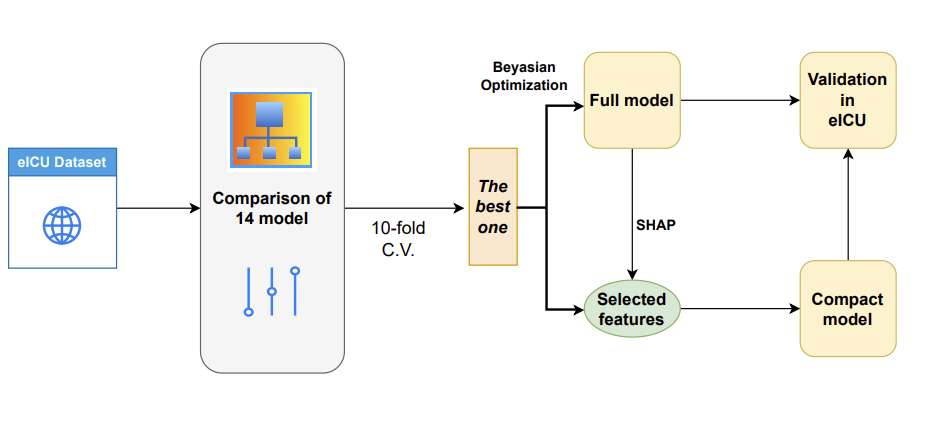
\includegraphics[width=0.9\linewidth]{../img/training.png}
    \caption{模型训练流程图}
    \label{fig:training}
\end{figure}

如图 \ref{fig:training} 所示,我们初步比较了 $14$ 种开源的模型训练后的预测表现,训练过程采用十折交叉验证。%
在每折验证集上计算准确度和受试者工作特征曲线下面积(AUC),并将其汇总以评估每种模型,%
选择精度最高、AUC 值最大的算法。随后利用贝叶斯优化算法对模型进行细粒度超参数调整,%
该算法是一种高效的约束全局优化工具,使用 bayes\_opt 开源工具包的函数实现。%
优化后的模型为本研究预测 PICS 的最佳模型,将其作为我们的完整模型。

变量对 PICS 预测的影响是使用 Python 的拓展包 SHAP 来测量的,%
该开源包使用基于验证集的博弈论方法评估每个特征的重要性。%
我们选择了 $15$ 个非常重要且在临床环境中尽可能容易收集的变量,%
然后基于所选变量训练一个紧凑的模型用于 PICS 预测,%
虽然该模型不如完整模型准确,但在临床中可能更实用。


\section{模型结果}

\NewDocumentCommand\MyCompare{m m m}{($#1$\ vs.\ $#2$, $p<#3$)}

\subsection{基准特征}

从eICU数据库中共提取出$100,308$条数据,包含$17,729$名不同的脓毒症患者。%
其中,$3,866\,(3.85\%)$条数据为正例,$96,442\,(96.15\%)$条数据为反例。

经过比较,正例拥有更长的ICU入住天数\MyCompare{21.067}{10.852}{0.001},%
更少的血浆蛋白\MyCompare{2.109}{2.520}{0.001},%
更少的淋巴细胞数目\MyCompare{9.931}{12.473}{0.001},%
更高的心率\MyCompare{93.337}{88.458}{0.001},%
更高的呼吸频率\MyCompare{21.814}{21.019}{0.001},%
更少的血清总蛋白\MyCompare{5.578}{5.928}{0.001},%
更低的红细胞比容\MyCompare{27.808}{29.888}{0.001},%
更少的肌酸酐\MyCompare{1.489}{1.610}{0.001},%
更高的白细胞计数\MyCompare{13.218}{12.189}{0.001},%
更多的血小板\MyCompare{260.259}{226.342}{0.001},%
更低的平均动脉压\MyCompare{79.727}{82.055}{0.001}。

\subsection{模型比较}

\begin{table}[htbp]
    \centering
    \scriptsize
    \begin{threeparttable}
        \begin{tabular}{clcc}
            \toprule
            排名 & 模型名称                         & 平均准确率               & 平均AUC\tnote{1}      \\
            \midrule
            1  & CatBoost                     & $0.996 (\pm 0.001)$ & $0.996 (\pm 0.001)$ \\
            2  & Light Gradient Boosting      & $0.995 (\pm 0.001)$ & $0.996 (\pm 0.001)$ \\
            3  & Extreme Gradient Boosting    & $0.995 (\pm 0.001)$ & $0.994 (\pm 0.002)$ \\
            4  & Hist Gradient Boosting       & $0.994 (\pm 0.002)$ & $0.996 (\pm 0.002)$ \\
            5  & Ada Boost                    & $0.993 (\pm 0.002)$ & $0.995 (\pm 0.002)$ \\
            6  & Decision Tree                & $0.989 (\pm 0.002)$ & $0.949 (\pm 0.013)$ \\
            7  & Multi-Layer Perceptron       & $0.982 (\pm 0.004)$ & $0.975 (\pm 0.008)$ \\
            8  & SVM (RBF Kernel)             & $0.973 (\pm 0.003)$ & $0.957 (\pm 0.011)$ \\
            9  & Logistic                     & $0.966 (\pm 0.007)$ & $0.956 (\pm 0.012)$ \\
            10 & Extra Trees                  & $0.961 (\pm 0.006)$ & $0.977 (\pm 0.006)$ \\
            11 & Naive Bayes                  & $0.961 (\pm 0.006)$ & $0.689 (\pm 0.034)$ \\
            12 & Ridge                        & $0.961 (\pm 0.007)$ & $0.952 (\pm 0.013)$ \\
            13 & Linear Discriminant Analysis & $0.961 (\pm 0.010)$ & $0.952 (\pm 0.013)$ \\
            14 & K-Nearest Neighbours         & $0.951 (\pm 0.006)$ & $0.544 (\pm 0.025)$ \\
            \bottomrule
        \end{tabular}
        \begin{tablenotes}
            \tiny
            \item[1] AUC:Area Under Curve,接受者操作特性曲线下与坐标轴围成的面积。
        \end{tablenotes}
    \end{threeparttable}
    \caption{$14$种模型的交叉验证结果比较(按平均准确率排序)}
    \label{table:model-comparison}
\end{table}

用提取出的数据训练预测模型,各种模型的交叉验证结果如表\ref{table:model-comparison}所示。%
Logistic回归表现良好(平均准确率:$0.966$,平均AUC:$0.956$),%
而集成学习方法拥有更高的平均准确率和平均AUC。%
其中,CatBoost的预测结果最好(平均准确率:$0.996$,平均AUC:$0.996$),%
故选择CatBoost进入下一步。

\subsection{完整模型与紧凑模型}

\begin{figure}[htbp]
    \centering
    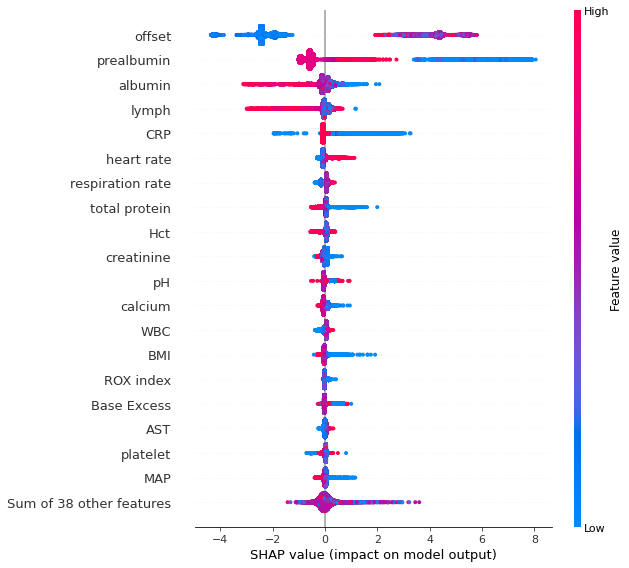
\includegraphics[width=0.9\linewidth]{../img/eicu_full_shap_beeswarm_20.png}
    \caption{完整模型中各变量的平均SHAP值比较}
    \label{figure:full-shap}
\end{figure}

根据预测结果比较,选择含$57$个输入变量的CatBoost模型为完整模型。%
计算完整模型中各变量的平均SHAP值,结果如图\ref{figure:full-shap}所示。%
此摘要图展示了各个变量对预测结果的影响情况分布。%
例如,ICU入住天数(offset)对结果影响明显,且ICU入住天数越长,发生ICU综合症的概率越大。

TODO:

\subsection{性能分析}

TODO:

\subsection{模型解释}

TODO:

\subsection{H5预测工具}

TODO:



\section{结论}

总之,本研究比对了 $14$ 种模型的交叉验证结果,认为 CatBoost 模型最适合本课题,%
且基于 CatBoost 训练了一个完整模型与一个紧凑模型。其中,完整模型预测相对更精确,%
而紧凑模型在临床上更加简易实用,二者均可以比较准确预测脓毒症患者次日诱发 PICS 的风险。


\appendix
\begin{thebibliography}{9}
    \bibitem{sepsis}
    王锦权,金朋.脓毒症患者病情及预后评估的临床意义[J].安徽医学,2022,43(08):869-872.
    \bibitem{pics}
    韩雪妹,王日兴.脓毒症相关持续性炎症-免疫抑制-分解代谢综合征的研究进展%
    [J].感染、炎症、修复,2021,22(03):171-174.
    \bibitem{pics-conditions}
    李盼,马莉.持续性炎症-免疫抑制-分解代谢综合征发病机制及诊疗的新进展%
    [J].中华重症医学电子杂志(网络版),2020,6(03):318-321.
    \bibitem{micro-rna}
    杨蓉,王鹏,屈文静.脓毒症患者继发持续性炎症-免疫抑制-分解代谢综合征的影响因素%
    及预测模型构建[J].海南医学,2021,32(17):2182-2185.
    \bibitem{pics-prediction-methods}
    周倩钰.基于eICU数据库急性胰腺炎严重程度及预后预测指标的研究%
    [D].华中科技大学,2022.DOI:10.27157/d.cnki.ghzku.2022.005907.
    \bibitem{eicu}
    Pollard Tom J;;Johnson Alistair E W;;Raffa Jesse D;;Celi Leo A;;Mark Roger G;;Badawi Omar.
    The eICU Collaborative Research Database, a freely available multi-center database for critical care research.
        [J].Scientific data,2018(1).
\end{thebibliography}

\end{document}
